\scanpage{3}
\mspage{1}
\margin{\textcircled{I}\par\uline{Modèles \inserted{$R$-}modérés} \deleted{et espaces}\inserted{ens} \deleted{modérés}}
\[
\forall n\in\mathbb N^*,\qquad\mathcal M_n\subset\mathcal P(R^n)
\]
\textcircled{\scriptsize$M1$} $\forall u:[1,n]\longrightarrow[1,m]$, d'où $u^*:R^m\longrightarrow R^n$, on a
\[
u^*(\mathcal M_m)\subset\mathcal M_n\qquad\text{i.e.}\quad\forall A\in\mathcal M_m,\text{ on a }u^*(A)\in\mathcal M_n.
\]
\textcircled{\scriptsize$M2$} $\forall u:[1,n]\longrightarrow[1,m]$ \uline{surjectif}, d'où $u^*:R^m\hookrightarrow R^n$ injectif, on a
\[
u^{*-1}(\mathcal M_n)\subset\mathcal M_m\qquad\text{i.e.}\quad\forall \inserted{B}\in\mathcal M_n,\text{ on a }u^{*-1}(\deleted{A}\inserted{B})\in\mathcal M_m.
\]
\margin{donc si on a $M1$, on trouve\par $A\in\mathcal M_m\Longleftrightarrow u_*(A)\in\mathcal M_n$}
\textcircled{\scriptsize$M3$} $\forall u:[1,n]\longrightarrow[1,m]$ d'où $u^*:R^m\longrightarrow R^n$, et pour $A\in\mathcal M_m$, $B\in\mathcal M_n$, on a
\[
u^{*-1}(B)\cap A\in\mathcal M_m
\]
\textcircled{\scriptsize$M4$} $\forall A\in\mathcal M_m$, $B\in\mathcal M_n$, on a (modulo $R^m\times R^n\simeq R^{m+n}$)
\[
A\times B\in\mathcal M_{m+n}.
\]

\uline{Commentaires} \textcircled{1} $M1)$ permet de définir, pour \deleted{tout} $I$ ens fini non vide, $\mathcal M_I\in\mathcal P(R^I)$, et alors on a des propriétés $M'1$ à $M'4$ pour les $\mathcal M_I$ et les $u:I\mathbin{-}J$.

\textcircled{2} : Pour avoir $M1$, il suffit de le supposer pour les \deleted{trois} cas :

a) $m=n$, $u\in\mathfrak S_n$

b) $m=n+1$, $u$ injectif (``op. face''), donc $u^*$ surjectif

c) $n=m+1$, $u$ surjectif \deleted{\unsure{(``op. dégénérescence'')}} \inserted{(``op dégénérescence'')} donc $u^*$ injectif

\deleted{et $\overline{\mathrm m}$ seulement les \unsure{opérat\textsuperscript{s}|opérations} stand.}

\margin{ou $\overline{\mathrm m}$ seulement les op. standard\par
$R^n\mathbin{-}R^{n+1},\ (x_1,\ldots,x_n)\longmapsto(x_1,\ldots,x_n,x_n)$\par
et\par
$R^{n+1}\mathbin{-}R^n,\ (x_1,\ldots,x_{n+1})\longmapsto(x_1,\ldots,x_n)$}

Pour avoir $M2$, il suffit de le supposer pour les op${}^{\mathrm{o}}$ de dégénérescences, \inserted{et $\overline{\mathrm m}$ seulement pour l'application \deleted{$\unsure{R^n\hookrightarrow R^{n+1}}$} \figure{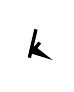
\begin{tikzpicture}[x=.12cm,y=.12cm,baseline=-.5ex]\draw[line width=1.2pt] (0,0)--(.7,3) (.45,1.1)--(1.6,.2)--(.3,.6)--(1.1,1.6);\end{tikzpicture}}}
\margin{\figure{
\begin{tikzpicture}[x=.12cm,y=.12cm]\draw[line width=1.2pt] (0,0)--(.7,3) (.45,1.1)--(1.6,.2)--(.3,.6)--(1.1,1.6);\end{tikzpicture}}\par
\figure{\begin{tikzpicture}[x=1cm,y=1cm]
\draw (-2.05,.95) .. controls (-.5,.92) and (2.1,1) .. (2.15,.25)
 .. controls (2.45,-.8) and (1.95,-1.05) .. (.1,-1.05)
 .. controls (-2.15,-1.02) and (-2.25,-.6) .. (-2.05,.95);
\node at (0,0) {$\begin{gathered}R^n\hookrightarrow R^{n+1}\\(x_1,\ldots,x_n)\deleted{\unsure{\longmapsto|x_n}}\\\longmapsto(x_1,\ldots,x_n,x_n)\end{gathered}$};
\end{tikzpicture}}}
Notons que $M1$, $M2$, $M4$ impliquent que les $\mathfrak S_n$ sont stables par intersection de deux
\[
A,B\in\mathfrak S_n\Longrightarrow A\cap B\in\mathfrak S_n
\]
\inserted{(moyennant $M1$, $M2$, $M4$)}
d'où résulte que pour avoir $M3$, il suffit de le prouver pour $u$ injectif, et $\overline{\mathrm m}$ seulement pour $u^*$ l'op. standard
\[
R^{n+1}\mathbin{-}R^n,\quad(x_1,\ldots,x_{n+1})\longmapsto(x_1,\ldots,x_n).
\]
\mspage{2}
